\documentclass[10pt]{beamer}

\usetheme{Madrid}
\usecolortheme{default}

% Base packages
%\usepackage{helvet}
\usepackage{amsthm,graphicx,xcolor,natbib,booktabs,tabularx,mathtools,subcaption}
\usepackage{unicode-math,mathrsfs}
\usepackage{amsmath,amssymb}
\usepackage{tikz,pgfplots}
\usetikzlibrary{arrows.meta, positioning, quotes}

%\usepackage[cache=false]{minted}
%\renewcommand{\theFancyVerbLine}{\sffamily\textcolor[rgb]{0.5,0.5,1.0}{\scriptsize\oldstylenums{\arabic{FancyVerbLine}}}}
%\definecolor{bg}{rgb}{.95,.95,.95}

% Font settings
\renewcommand{\familydefault}{\sfdefault}

% TikZ libraries
\usetikzlibrary{calc,positioning,backgrounds,decorations.pathreplacing}
\pgfplotsset{compat=1.14}

% Colors
\definecolor{deepblue}{RGB}{42,39,155}
\definecolor{lightpink}{RGB}{255,240,240}
\definecolor{lightgreen}{RGB}{240,255,240}
\definecolor{lightyellow}{RGB}{255,255,240}
\definecolor{codegray}{RGB}{245,245,245}
\definecolor{codegreen}{rgb}{0,0.6,0}
\definecolor{codepurple}{rgb}{0.58,0,0.82}

% Beamer settings
\setbeamercolor{title}{fg=white,bg=deepblue}
\setbeamercolor{frametitle}{fg=white,bg=deepblue}
\setbeamercolor{section in head/foot}{fg=white,bg=deepblue}

\setbeamertemplate{footline}[text line]{%
  \parbox{\linewidth}{\vspace*{-8pt}
  %\hfill\href{https://github.com/chang-ye-tu/fin}{https://github.com/chang-ye-tu/fin}
    \hfill
   \insertframenumber~/ \inserttotalframenumber}}
\setbeamertemplate{navigation symbols}{}%[only frame symbol]

\definecolor{foo}{rgb}{.2,.2,.7}
\AtBeginSection[]{
  \begin{frame}
  \vfill
  \centering
  \begin{beamercolorbox}[sep=8pt,center,shadow=true,rounded=true]{section page}
    \usebeamerfont{title}%
    {\color{foo} \insertsectionhead}\par%
  \end{beamercolorbox}
  \vfill
  \end{frame}
}

% https://tex.stackexchange.com/questions/30423/bibliography-in-beamer
\setbeamertemplate{bibliography entry title}{}
\setbeamertemplate{bibliography entry location}{}
\setbeamertemplate{bibliography entry note}{}

\newcommand{\ds}{\displaystyle}
\newcommand{\ie}{\;\Longrightarrow\;}
\newcommand{\ifff}{\;\Longleftrightarrow\;}
\newcommand{\mi}{\mathrm{i}}
\DeclareMathOperator*{\dom}{dom}
\DeclareMathOperator*{\codom}{codom}
\DeclareMathOperator*{\ran}{ran}
\newcommand{\floor}[1]{\lfloor #1 \rfloor}
\newcommand{\ceil}[1]{\lceil #1 \rceil}
\newcommand{\Set}[2]{\big\{ \ #1\ \big|\ #2\ \big\}}
\newcommand{\pdiff}[2]{\frac{\partial\hfil#1\hfil}{\partial #2}}
\newcommand{\vx}{\symbfup{x}}
\newcommand{\vd}{\symbfup{d}}
\newcommand{\vg}{\symbfup{g}}
\newcommand{\vH}{\symbfup{H}}
\newcommand{\va}{\symbfup{a}}
\newcommand{\vb}{\symbfup{b}}
\newcommand{\vbb}{\symbfup{\beta}}
\newcommand{\vS}{\symbfup{S}}
\newcommand{\vR}{\symbfup{R}}
\newcommand{\vV}{\symbfup{V}}
\newcommand{\ve}{\symbfup{e}}
\newcommand{\vr}{\symbfup{r}}
\newcommand{\vZero}{\symbfup{0}}

\DeclareMathOperator\prb{{\sf P}}
\DeclareMathOperator\expc{{\sf E}}
\DeclareMathOperator\var{var}
\DeclareMathOperator\cov{cov}
\DeclareMathOperator\cor{cor}
\DeclareMathOperator*{\argmax}{\arg\!\max}
\DeclareMathOperator*{\argmin}{\arg\!\min}
\DeclareMathOperator*{\im}{Im}
\DeclareMathOperator*{\re}{Re}
\DeclareMathOperator*{\conv}{conv}
\DeclareMathOperator*{\proj}{proj}
\DeclareMathOperator*{\tr}{tr}
\DeclareMathOperator*{\diag}{diag}
\DeclareMathOperator*{\epi}{epi}
\DeclareMathOperator*{\dist}{dist}
\DeclareMathOperator*{\inte}{int}
\DeclareMathOperator*{\relint}{relint}

\theoremstyle{definition}
\newtheorem*{dfn}{Definition}
\newtheorem*{prp}{Property}
\newtheorem*{thm}{Theorem}
\newtheorem*{ex}{Example}
\newtheorem*{prob}{Problem}
\newtheorem*{sol}{Solution}
\newtheorem*{prf}{Proof}
\usepackage{nicefrac}

\newcommand\scalemath[2]{\scalebox{#1}{\mbox{\ensuremath{\displaystyle #2}}}}

\title{Portfolio Optimization}
\author{}
\date{}

\begin{document}

\begin{frame}
\titlepage
\end{frame}

%\subsection*{Outline}
%\begin{frame}
%  \tableofcontents
%\end{frame}

\begin{frame}{Classical PO: Mean-Variance (MV) Criterion}
  \begin{itemize}[<+->]
    \item Assets evolve from time $0$ to time $1$ for one period
    \item $s$: \# of risky assets 
    \item $\vS_0\equiv(S_{1, 0}, S_{2, 0}, \ldots, S_{s, 0})^\top\not=\vZero$: the constant price vector at time $0$
    \item $\vS_1\equiv(S_{1, 1}, S_{2, 1}, \ldots, S_{s, 1})^\top$: the random price vector at time $1$
    \item $\vx\equiv(x_1, x_2, \ldots, x_s)^\top$: the proportion vector of the time-$0$ wealth invested in each asset; $\ds\sum_{i=1}^s x_i = 1$.
    \item $\vR\equiv(R_1, R_2, \ldots, R_s)^\top$: the random vector representing the rate of return on the assets; $\ds R_i = \frac{S_{i, 1}}{S_{i, 0}}$
    \item $w$: the (constant) wealth at time $0$
  \end{itemize}
\end{frame}

\begin{frame}{Classical PO: Mean-Variance (MV) Criterion}
  \begin{itemize}[<+->]
    \item $W$: the (random) wealth at time $1$; $\ds W = \bigg(\sum_{i=1}^s x_i R_i\bigg) w = \vx^\top\vR\,w$ \\(For asset $S_i$, $\ds\frac{x_i w}{S_{i, 0}}$ denotes the ``quantity'' allocated at time $0$; so at time $1$ this part of wealth becomes $\ds\frac{x_i w}{S_{i, 0}}\,S_{i, 1} = x_i R_i w$)  
    \item $\vr\equiv\expc{\vR} = (r_1, r_2, \ldots, r_s)^\top$: the (constant) mean vector of $\vR$; $\ds r_i = \expc{R_i}$
    \item $\vV\equiv\cov{\vR}\equiv\expc\{(\vR - \vr)(\vR - \vr)^\top\}$: the (constant) covariance matrix of $\vR$; $\vV$ is symmetric positive definite $s\times s$ matrix
    \item $\expc W = \expc\{\vx^\top\vR\} = \vx^\top\vr = \mu$
    \item $\sigma^2 = \var W = \var\{\vx^\top\vR\} = \expc\{\vx^\top(\vR - \vr)(\vR - \vr)^\top\vx\} = \vx^\top\vV\vx$
    \item ``For some fixed mean rate of return $\mu = \expc\{\vx^\top\vR\}$, try to minimize the variance $\sigma^2 = \var\{\vx^\top\vR\}$ of the return over portfolios $\vx$''
  \end{itemize}
\end{frame}

\begin{frame}{MV: All Risky Assets}
  \begin{align*}
    \min_{\vx}\,\frac{1}{2}\,\vx^\top\vV\vx\quad\text{s.t.}\quad\begin{cases}\vx^\top\ve = 1 \\\vx^\top\vr = \mu\end{cases}\quad \ve\equiv\underbrace{(1, 1, \ldots, 1)^\top}_{\text{$s$ items}}
  \end{align*}
  \onslide<+->
  \begin{itemize}[<+->]
    \item $\vV$ is symmetric, positive definite, so $\vV^{-1}$ also is
    \item Set $\ds\mathcal{L}\equiv\frac{1}{2}\,\vx^\top\vV\vx + \lambda\,(1 - \vx^\top\ve) + \nu\,(\mu - \vx^\top\vr)$ with Lagrange multipliers $\lambda$, $\nu$
    \item By $\ds\frac{\partial\mathcal{L}}{\partial\vx} = \vV\vx - \lambda\,\ve - \nu\,\vr = 0\ie\vx = \lambda\,\vV^{-1}\ve + \nu\,\vV^{-1}\vr$ $\ds\ie\vx^\top = \lambda\,\ve^\top\left(V^{-1}\right)^\top + \nu\,\vr^\top\left(V^{-1}\right)^\top = \lambda\,\ve^\top\vV^{-1} + \nu\,\vr^\top\vV^{-1}$ 
    \item Substitute into $\ds\begin{cases}\vx^\top\ve = 1 \\\vx^\top\vr = \mu\end{cases}\ie\begin{cases}\lambda\,\ve^\top\vV^{-1}\ve + \nu\,\vr^\top\vV^{-1}\ve = 1 \\ \lambda\,\ve^\top\vV^{-1}\vr + \nu\,\vr^\top\vV^{-1}\vr = \mu\end{cases}$
  \end{itemize}
\end{frame}

\begin{frame}
  \begin{itemize}[<+->]
    \item Set $\alpha = \ve^\top\vV^{-1}\ve,\;$ $\beta = \vr^\top\vV^{-1}\ve = \ve^\top\vV^{-1}\vr,\;$ $\gamma = \vr^\top\vV^{-1}\vr,\;$ $\delta\equiv\alpha\gamma - \beta^2\;$, then
      \onslide<+->
      \begin{align*}
        \begin{cases}\lambda\,\ve^\top\vV^{-1}\ve + \nu\,\vr^\top\vV^{-1}\ve = 1 \\ \lambda\,\ve^\top\vV^{-1}\vr + \nu\,\vr^\top\vV^{-1}\vr = \mu\end{cases}
      \end{align*}
      becomes 
      \onslide<+->
      \begin{align*}\begin{cases}\lambda\alpha + \nu\beta = 1 \\ \lambda\beta + \nu\gamma = \mu\end{cases}
      \end{align*}
      \onslide<+->
      Solutions: $\ds\lambda = \frac{\gamma - \beta\mu}{\delta},\;$ $\ds\gamma = \frac{\alpha\mu - \beta}{\delta}$
    \item If $\vr\not=c\,\ve$, $c\in\mathbb{R}$, then from the positive-definiteness of $\vV^{-1}$ 
      \onslide<+->
      \begin{align*}
        &(\vr - c\,\ve)^\top\vV^{-1}(\vr - c\,\ve) > 0 \\
        &\ie\vr^\top\vV^{-1}\vr - c\,\vr^\top\vV^{-1}\ve - c\,\ve\vV^{-1}\vr + c^2\,\ve^\top\vV^{-1}\ve^\top > 0 \\
        &\ie \gamma-2\,c\,\beta + c^2\,\alpha > 0 \\
        &\ie-\delta = \beta^2 - \gamma\alpha < 0
      \end{align*}
  \end{itemize}
\end{frame}

\begin{frame}
  \begin{itemize}[<+->]
    \item The relation of $\sigma$ with $\mu$: 
      \onslide<+->
      \begin{align*}
        \sigma^2 &= \vx^\top\vV\vx = \vx^\top\vV(\lambda\vV^{-1}\ve + \nu\vV^{-1}\vr) = \lambda(\vx^\top\ve) + \nu(\vx^\top\vr) \\
        &= \lambda + \nu\mu = \frac{\gamma - \beta\mu}{\delta} + \nu\frac{\alpha\mu-\beta}{\delta} = \frac{\alpha\mu^2 - 2\beta\mu + \gamma}{\delta}\\
        &\ie\frac{\sigma^2}{\left(\frac{1}{\sqrt{\alpha}}\right)^2} - \frac{\left(\mu - \frac{\beta}{\alpha}\right)^2}{\left(\frac{\sqrt{\delta}}{\alpha}\right)^2} = 1
      \end{align*}
    \item Recall the standard form of hyperbola $(x, y)$ 
      \onslide<+->
      \begin{align*}
        \text{equation:}\quad &\frac{(x - h)^2}{a^2} - \frac{(y - k)^2}{b^2} = 1 \\
        \text{asymptotes:}\quad &(y - k) =\pm\frac{b}{a}(x - h)
      \end{align*}
    \item Here we have $(\sigma, \mu)$ with $\ds a = \frac{1}{\sqrt{\alpha}}$, $\ds b = \frac{\sqrt{\delta}}{\alpha}$, $\ds h = 0$, $\ds k = \frac{\beta}{\alpha}$, the asymptotes are $\ds\left(\mu - \frac{\beta}{\alpha}\right) = \pm\frac{\frac{\sqrt{\delta}}{\alpha}}{\frac{1}{\sqrt{\alpha}}}\sigma$ $\ie$ $\ds \mu = \frac{\beta}{\alpha} \pm\sqrt{\frac{\delta}{\alpha}}\sigma$
  \end{itemize}
\end{frame}

\begin{frame}
\begin{itemize}[<+->]
  \item Global minimum-variance portfolio $\vx_g$
    \begin{itemize}
      \item First find $\mu_g$ that minimizes $\ds\sigma^2 = \frac{\alpha\mu^2 - 2\beta\mu + \gamma}{\delta}$: By differentiation $\ds 2\alpha\mu_g - 2\beta = 0\ie\mu_g = \frac{\beta}{\alpha}$
      \item $\ds\lambda_g = \frac{\gamma - \beta\mu_g}{\delta} = \frac{\gamma-\beta\frac{\beta}{\alpha}}{\delta} = \frac{\gamma\alpha - \beta^2}{\alpha\delta} = \frac{1}{\alpha}$ \\ $\ds\nu_g = \frac{\alpha\mu_g - \beta}{\delta} = \frac{\beta - \beta}{\delta} = 0$ \\ so $\ds\vx_g = \lambda_g\,\vV^{-1}\ve + \nu_g\,\vr^\top\vV^{-1} = \frac{1}{\alpha}\vV^{-1}\ve$
    \end{itemize}
  \item Diversified portfolio: define $\ds\vx_d\equiv\frac{1}{\beta}\vV^{-1}\vr$, then the expected return $\ds\mu_d = \vx^\top_d\vr = \frac{1}{\beta}\vr^\top\vV^{-1}\vr = \frac{\gamma}{\beta}$
  \item $\ds\vx = \lambda\vV^{-1}\ve + \nu\vV^{-1}\vr = \lambda\,\alpha\,\vx_g + \nu\,\beta\,\vx_d$, so {\bf every portfolio is the convex combination of $\vx_g$ and $\vx_d$}: note that $\ds\lambda\alpha + \nu\beta = 1$ (constraint $\ds\vx^\top\ve = 1$) ! 
\end{itemize}
\onslide<+->
\begin{thm}[Mutual Fund Theorem]
  Any minimum-variance portfolio is equivalent to investing in the convex combination of $\vx_g$ and $\vx_d$.
\end{thm}
\end{frame}

\begin{frame}
  \begin{figure}[!htbp]
    \centering
    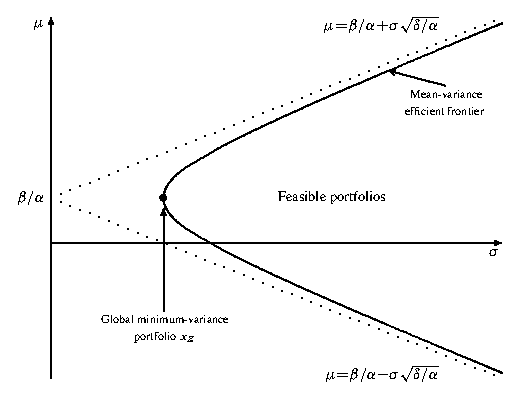
\includegraphics[scale=1.1,page=1]{fig/sfm.pdf}
    \caption{The Case of All Risky Assets}
    \label{fig:mv1}
  \end{figure}
\end{frame}

\begin{frame}
  \begin{thm}
    Diversified portfolio $\vx_d$ is the portfolio that maximize $\ds s(\vx)\equiv\frac{\vx^\top\vr}{\sqrt{\vx^\top\vV\vx}}$.
  \end{thm}
  \onslide<+->
  \begin{prf}
    \begin{itemize}[<+->]
      \item Maximize $s(\vx)$ $\equiv$ maximize $\log(s(\vx))$ s.t. $\ds\vx^\top\ve = 1$ 
      \item Change of variable: $\ds\vx^\top\vr = \mu$ $\ds\ie\log(s(\vx)) = \log\frac{\mu}{\sqrt{\frac{\alpha\mu^2 - 2\beta\mu + \gamma}{\delta}}} \equiv f(\mu)$ with $\mu > 0$
      \item $\ds f'(\mu) = \frac{\gamma - \beta\mu}{\mu\left(\alpha\left(\mu - \frac{\beta}{\alpha}\right)^2 + \frac{\delta}{\alpha}\right)} = 0$ at $\ds\mu = \frac{\gamma}{\beta} = \mu_d$
    \end{itemize}
  \end{prf}

  \begin{itemize}[<+->]
    \item The covariance between the return of the global mininum-variance portfolio and other minimum-variance portfolio is constant: $\ds\cov(\vx^\top_g\vR, \vx^\top\vR) = \vx^\top_g\vV\vx = \vx^\top_g\vV(\lambda\,\vV^{-1}\ve + \nu\,\vV^{-1}\vr) = \lambda\,\vx^\top_g\ve + \nu\,\vx^\top_g\vr$ \\ $=$ $\ds\frac{\lambda}{\alpha}\,\ve^\top\vV^{-1}\ve + \frac{\nu}{\alpha}\,\ve^\top\vV^{-1}\vr = \frac{\lambda\,\alpha + \nu\,\beta}{\alpha} = \frac{1}{\alpha}$
  \end{itemize}
\end{frame}

\begin{frame}
\begin{figure}[!htbp]
  \centering
  \includegraphics[scale=1.1,page=2]{fig/sfm.pdf}
  \caption{The Diversified Portfolio}
  \label{fig:mv2}
\end{figure}
\end{frame}

\begin{frame}{MV: All But One Risky Assets}
\onslide<+->
\noindent WLOG add riskless asset $0$ with constant return $r_0$; the portfolio becomes $(x_0, x_1, x_2, \ldots, x_s)^\top$ 
\onslide<+->
\begin{align*}
  \min_{x_0, \vx}\,\frac{1}{2}\,\vx^\top\vV\vx\quad\text{s.t.}\quad\begin{cases} x_0 + \vx^\top\ve = 1 \\ x_0 r_0 + \vx^\top\vr = \mu\end{cases}\quad\ve\equiv\underbrace{(1, 1, \ldots, 1)^\top}_{\text{$s$ items}}
\end{align*}
\begin{itemize}[<+->]
  \item Set $\ds\overline{\mathcal{L}}\equiv\frac{1}{2}\,\vx^\top\vV\vx + \overline{\lambda}\,(1 - x_0 - \vx^\top\ve) + \overline{\nu}\,(\mu - x_0 r_0 \vx^\top\vr)$ with Lagrange multipliers $\overline{\lambda}$, $\overline{\nu}$
  \item By $\ds\frac{\partial\overline{\mathcal{L}}}{\partial\vx} = \vV\vx - \overline{\lambda}\,\ve - \overline{\nu}\,\vr = 0\ie\vx = \overline{\lambda}\,\vV^{-1}\ve + \overline{\nu}\,\vV^{-1}\vr$, \\ so $\ds\vx^\top = \overline{\lambda}\,\ve^\top\left(V^{-1}\right)^\top + \overline{\nu}\,\vr^\top\left(V^{-1}\right)^\top = \overline{\lambda}\,\ve^\top\vV^{-1} + \overline{\nu}\,\vr^\top\vV^{-1}$
  \item By $\ds\frac{\partial\overline{\mathcal{L}}}{\partial x_0} = -\overline{\lambda} - \overline{\nu}r_0 = 0\ie\overline{\nu} = -\frac{\overline{\lambda}}{r_0}$
\end{itemize}

\end{frame}

\begin{frame}
\begin{itemize}[<+->]
  \item $\ds\begin{cases}x_0 + \vx^\top\ve = 1 \\ x_0 r_0 + \vx^\top\vr = \mu\end{cases}\!\!\!\!\ie\begin{cases}x_0 + \overline{\lambda}\,\ve^\top\vV^{-1}\ve + \overline{\nu}\,\vr^\top\vV^{-1}\ve = 1 \\ x_0 r_0 + \overline{\lambda}\,\ve^\top\vV^{-1}\vr + \overline{\nu}\,\vr^\top\vV^{-1}\vr = \mu\end{cases}$ 
  \item Set $\alpha = \ve^\top\vV^{-1}\ve,\;$ $\beta = \vr^\top\vV^{-1}\ve = \ve^\top\vV^{-1}\vr,\;$ $\gamma = \vr^\top\vV^{-1}\vr,\;$ $\delta\equiv\alpha\gamma - \beta^2\;$, the above becomes
    \begin{align*}
      \begin{cases}x_0 + \overline{\lambda}\alpha + \overline{\nu}\beta = x_0 + \overline{\lambda}\alpha - \frac{\overline{\lambda}}{r_0}\beta = 1 \\ x_0 r_0 + \overline{\lambda}\beta + \overline{\nu}\gamma = x_0 r_0 + \overline{\lambda}\beta - \frac{\overline{\lambda}}{r_0}\gamma = \mu\end{cases}
    \end{align*}
    with solutions $\ds x_0 = \frac{\alpha\mu r_0 - \beta r_0 + \gamma - \beta\mu}{\epsilon^2}$, $\ds\overline{\lambda} = \frac{(r_0 - \mu)r_0}{\epsilon^2}$, \\ $\ds\overline{\nu} = -\frac{r_0 - \mu}{\epsilon^2}$, where $\ds\epsilon^2 = \alpha r_0^2 - 2\beta r_0 + \gamma = \alpha\Big(r_0 - \frac{\beta}{\alpha}\Big)^2 + \frac{\delta}{\alpha}$ 
  \item The relation of $\sigma$ with $\mu$
    \begin{align*}
      \sigma^2 &= \vx^\top\vV\vx = \vx^\top\vV(\overline{\lambda}\vV^{-1}\ve + \overline{\nu}\vV^{-1}\vr) = \overline{\lambda}(\vx^\top\ve) + \overline{\nu}(\vx^\top\vr) \\ 
      &= \overline{\lambda}(1 - x_0) + \overline{\nu}(\mu - x_0 r_0) = \overline{\lambda} + \overline{\nu}\mu = \frac{(\mu - r_0)^2}{\epsilon^2}
    \end{align*}
\end{itemize}
\end{frame}

\begin{frame}
\begin{figure}[!htbp]
  \centering
  \includegraphics[scale=1,page=3]{fig/sfm.pdf}
  \caption{The Case of All But One Risky Assets}
  \label{fig:mv3}
\end{figure}
\end{frame}

\begin{frame}
\onslide<+->
\begin{prp}
  If $\ds r_0 < \frac{\beta}{\alpha}$, then $\mu = r_0 + \epsilon\sigma$ touches the hyperbola $\ds\sigma^2 = \frac{\alpha\mu^2 - 2\beta\mu + \gamma}{\delta}$ at $\ds\Big(\frac{\epsilon}{\beta - \alpha r_0}, \frac{\gamma - \beta r_0}{\beta - \alpha r_0}\Big)$
\end{prp}
\onslide<+->

\begin{prf}
  On $\sigma-\mu$ plane the slope of the tangent is obtained by implicit differentiation of $\ds\sigma^2 = \frac{\alpha\mu^2 - 2\beta\mu + \gamma}{\delta}$ w.r.t $\sigma$ (let $\ds\mu\equiv\mu(\sigma)$): $\ds 2\sigma = \frac{2\alpha\mu\mu' - 2\beta\mu'}{\delta}$ $\ie$ $\ds\mu' = \frac{\delta\sigma}{\alpha\mu - \beta}$. The tangent line is $\ds\mu = r_0 + \epsilon\sigma$ with slope $\epsilon$, so $\ds\epsilon$ $=$ $\ds\frac{\delta\sigma}{\alpha\mu - \beta}$ $\ie$ $\ds\delta\sigma = \alpha\mu\epsilon - \beta\epsilon$ $\ie$ $\ds\ds\delta\sigma = \alpha\epsilon(r_0 + \epsilon\sigma) - \beta\epsilon$ $\ie$ $\ds (\delta - \alpha\epsilon^2)\sigma = \epsilon(\alpha r_0 - \beta)$. Note that $\ds\epsilon^2 = \alpha r_0^2 - 2\beta r_0 + \gamma = \alpha\Big(r_0 - \frac{\beta}{\alpha}\Big)^2 + \frac{\delta}{\alpha}$, so $\ds\sigma$ $=$ $\ds\frac{\epsilon(\alpha r_0 - \beta)}{\delta - \alpha\epsilon^2}$ $=$ $\ds\frac{\epsilon(\alpha r_0 - \beta)}{-\alpha^2\big(r_0 - \frac{\beta}{\alpha}\big)^2} = \frac{\epsilon}{\beta - \alpha r_0}$, $\ds\mu = r_0 + \epsilon\frac{\epsilon}{\beta - \alpha r_0}$ $=$ $\ds\frac{\beta r_0 - \alpha r_0^2 + \epsilon^2}{\beta - \alpha r_0}$ $=$ $\ds\frac{\gamma - \beta r_0}{\beta - \alpha r_0}$.
\end{prf}
\end{frame}

\begin{frame}
  \begin{itemize}[<+->]
    \item Define the tangency portfolio
      \onslide<+->
      \begin{align*}
        \ds\vx_t = \frac{1}{\beta-\alpha r_0}\vV^{-1}(\vr - r_0\ve) = \frac{\beta}{\beta - \alpha r_0}\vx_d - \frac{\alpha r_0}{\beta - \alpha r_0}\vx_g
      \end{align*}
    \item $\ds\vx = \overline{\lambda}\vV^{-1}\ve + \overline{\nu}\vV^{-1}\vr = \overline{\nu}\vV^{-1}(\vr - r_0\ve)\equiv(1 - x_0)\vx_t$
    \item $\ds\ve^\top\vx_t = \frac{\beta}{\beta - \alpha r_0}\ve^\top\vx_d - \frac{\alpha r_0}{\beta - \alpha r_0}\ve^\top\vx_g = \frac{\beta}{\beta - \alpha r_0} - \frac{\alpha r_0}{\beta - \alpha r_0} = 1$
    \item $\ds\mu_t = \vx^\top_t\vr = \vr^\top\vx_t = \frac{\beta}{\beta - \alpha r_0}\vr^\top\vx_d - \frac{\alpha r_0}{\beta - \alpha r_0}\vr^\top\vx_g$ \\$\ds = \frac{\beta}{\beta - \alpha r_0}\mu_d - \frac{\alpha r_0}{\beta - \alpha r_0}\mu_g = \frac{\gamma - \beta r_0}{\beta - \alpha r_0}$ for $\ds\mu_d = \frac{\gamma}{\beta}$, $\ds\mu_g = \frac{\beta}{\alpha}$
  \end{itemize}
\end{frame}

\begin{frame}
  \onslide<+->
  \begin{thm}
    Tangency portfolio $\vx_t$ is the portfolio that maximize $\ds s(\vx)\equiv\frac{\vx^\top\vr - r_0}{\sqrt{\vx^\top\vV\vx}}$.
  \end{thm}
  \begin{prf}
    \begin{itemize}[<+->]
      \item Maximize $s(\vx)$ $\equiv$ maximize $\log(s(\vx))$ s.t. $\ds\vx^\top\ve = 1$ 
      \item Change of variable $\vx^\top\vr = \mu$ $\ds\ie\log(s(\vx)) = \log\frac{\mu - r_0}{\sqrt{\frac{\alpha\mu^2 - 2\beta\mu + \gamma}{\delta}}}\equiv f(\mu)$ with $\mu > r_0$
      \item $\ds f'(\mu) = \frac{(\gamma - \beta r_0) - (\beta - \alpha r_0)\mu}{(\mu - r_0)\left(\alpha\mu^2 - 2\beta\mu + \gamma\right)} = 0$ at $\ds\mu = \frac{\gamma - \beta r_0}{\beta - \alpha r_0} = \mu_t$.
    \end{itemize}
  \end{prf}
\end{frame}

\begin{frame}{Mean-Variance Pricing Equation}
  \begin{itemize}[<+->]
    \item $\ds\vV = \expc\big\{(\vR - \vr)(\vR - \vr)^\top\big\} = \expc\big\{\vR\,\vR^\top - \vR\,\vr^\top - \vr\,\vR^\top + \vr\,\vr^\top\big\} = \expc\big\{\vR\,\vR^\top - \vR\,\vr^\top\big\}$
    \item $\ds\cov(R_i, \vx^\top_t\vR) = \expc\big\{(R_i - r_i)(\vx^\top_t\vR - \vx^\top_t\vr)\big\} = \expc\big\{R_i\,\vx^\top_t\vR - R_i\,\vx^\top_t\vr - r_i\,\vx^\top_t\vR + r_i\,\vx^\top_t\vr\big\} = \expc\big\{R_i\,\vx^\top_t\vR - R_i\,\vx^\top_t\vr\} = \expc\big\{R_i\,\vR^\top\vx_t - R_i\,\vr^\top\vx_t\}$
    \item $\ds\vV\vx_t = \expc\big\{\vR\,\vR^\top\vx_t - \vR\,\vr^\top\vx_t\big\}$
    \item $\ds(\vV\vx_t)_i = \frac{1}{\beta - \alpha r_0}(r_i - r_0)$; 
    \item $\ds\var(\vx^\top_t\vR) = \expc\{\vx^\top_t\vR\cdot(\vx^\top_t\vR)^\top\} - (\expc\{\vx^\top_t\vR\})^2$ $=$ $\ds\expc\big\{\vx^\top_t\vR\,\vR^\top\vx_t\big\} - \expc\big\{\vx^\top_t\vR\big\}\expc\big\{\vR^\top\vx_t\big\}$ $=$ $\ds\expc\big\{\vx^\top_t\vR\,\vR^\top\vx_t\big\} - \vx^\top_t\vr\,\vr^\top\vx_t$ $=$ $\ds\vx^\top_t\expc\big\{\vR\,\vR^\top - \vr\,\vr^\top\big\}\vx_t$ $=$ $\ds\vx^\top_t V\vx_t = \frac{\mu_t - r_0}{\beta - \alpha r_0}$. 
    \item $\ds\beta_{i, t} = \frac{\cov(R_i, \vx^\top\vR)}{\var(\vx^\top\vR)} = \cor(R_i, \vx^\top\vR)\sqrt{\frac{\var{R_i}}{\var(\vx^\top\vR)}}$; define $\ds\vbb_t\equiv(\beta_{1, t}, \beta_{2, t}, \ldots, \beta_{s, t})^\top$ 
    \item $\ds\vbb_t = \frac{1}{\mu_t-r_0}(\vr - r_0\ve)$ $\ie$ $\ds\vr = r_0\ve + (\mu_t - r_0)\vbb_t$ 
  \end{itemize}
\end{frame}

\begin{frame}{Mean-Variance Analysis and Expected Utility}
  \begin{itemize}[<+->]
    \item Define $\ds f(\sigma,\mu) = \expc v(W)$ where $\ds W = (x_0 r_0 + \vx^\top\vR)w$, $\ds\sigma^2 = \vx^\top\vV\vx$, $\ds\mu = x_0 r_0 + \vx^\top\vr = \vx^\top(\vr - r_0\ve)$  
    \item Assume that $\ds\frac{\partial f}{\partial\sigma} < 0$, $\ds\frac{\partial f}{\partial\mu} > 0$ with $x_0 + \vx^\top\ve = 1$, perform $\ds\max_{\vx}f\left(\sqrt{\vx^\top\vV\vx}, r_0 + \vx^\top(\vr - r_0\ve)\right)$
    \item $\ds\frac{\partial f}{\partial\vx} = \frac{1}{\sigma}\frac{\partial f}{\partial\sigma}\,\vV\vx + \frac{\partial f}{\partial\mu}(\vr - r_0\ve) = 0$ $\ie$ $\ds\vx = -\frac{\sigma\frac{\partial f}{\partial\mu}}{\frac{\partial f}{\partial\sigma}}\vV^{-1}(\vr - r_0\ve)\propto\vx_t$
    \item Example:
      \begin{itemize}
        \item For quadratic utility $\ds v(x) = ax + bx^2$ where $a, b\in\mathbb{R}$, $b\leqslant 0$: $\ds\expc v(W) = \expc v((x_0 r_0 + \vx^\top\vR)w) = aw\mu + bw^2(\mu^2 + \sigma^2) = f(\sigma, \mu)$
        \item For normally distributed returns $\ds\vR\sim N(\vr, \vV)$, $\ds\vx^\top\vR\sim N(\vx^\top\vr, \vx^\top V\vx)$: $\ds\expc v(W) = \expc v((\mu + \sigma Y) w)$, where $\ds Y\sim N(0, 1)$ 
      \end{itemize}
  \end{itemize}
\end{frame}

\begin{frame}
\begin{figure}[!htbp]
  \centering
  \includegraphics[scale=1.1,page=4]{fig/sfm.pdf}
  \caption{Determining the Utility-Maximizing Portfolio}
  \label{fig:mv4}
\end{figure}
\end{frame}

\begin{frame}{Equilibrium: The Capital-Asset Pricing Model}
  \begin{itemize}[<+->]
    \item Investors indexed by $\ds j\in\mathcal{J}$, each with proportions of wealth $x_{0, j}$ and $\ds\vx_j = (x_{1, j},\,x_{2, j},\,\ldots,\,x_{s, j})^\top$ 
    \item When each investor $j$ has the utility function as above, the optimal $\ds\vx_j$ $\propto$ $\ds\vx_t$ $\ie$ $\ds\vx_j = (1 - x_{0, j})\,\vx_t$ $\forall j\in\mathcal{J}$
    \item The total value of the demand for risky asset $i$: $\ds\sum_{j\in\mathcal{J}} w_j x_{i, j} = \Big(\sum_{j\in\mathcal{J}}(1 - x_{0, j})w_j\Big)(\vx_t)_i$ 
    \item \emph{Market portfolio} of risky assets $\vx_m$: $\ds (\vx_m)_i\equiv\frac{\text{The total value of the supply of risky asset $i$}}{\text{The total value of the supply of all risky assets}}$; $\vx^\top_m\ve = 1$
    \item In equilibrium $\ds(\vx_m)_i =  \frac{\Big(\sum_{j\in\mathcal{J}}(1 - x_{0, j})w_j\Big)(\vx_t)_i}{\sum_{j\in\mathcal{J}}\sum_{k=1}^s w_j x_{k, j}} = \frac{\Big(\sum_{j\in\mathcal{J}}(1 - x_{0, j})w_j\Big)(\vx_t)_i}{\Big(\sum_{j\in\mathcal{J}}(1 - x_{0, j})w_j\Big)\sum_{k=1}^s(\vx_t)_k} = (\vx_t)_i$, since $\vx^\top_t\ve = 1$
    \item $\vr = r_0\ve + (\mu_m - r_0)\vbb_m$, $\vbb_m\equiv(\beta_{1, m}, \beta_{2, m}, \ldots, \beta_{s, m})^\top$, $\ds\beta_{i, m} = \frac{\cov(R_i, \vx^\top_m\vR)}{\var(\vx^\top_m\vR)}$ --- capital-asset-pricing equation
  \end{itemize}
\end{frame}

\section{Problems and Solutions}

\begin{frame}{Problem}
  Suppose that an investment $X$ has either (i) the uniform distribution $U[0, 2\mu]$ or (ii) the exponential distribution with $\expc X = \mu$, and the investor has a utility function which is either (a) logarithmic, $v(x) = \log x$ (b) power form, $v(x) = x^\theta$. Show that both the compensatory risk premium and the investment risk premium are proportional to $\mu$ in all 4 possible cases.
\end{frame}

\begin{frame}[fragile]
  \frametitle{Solution}
  \begin{itemize}[<+->]
    \item For distributions (i)(ii) of $X$, the r.v. $\ds Y\equiv\frac{X}{\mu}$ does not depend on $\mu$, so $\ds\expc v(X + \alpha) = v(\mu)$ for the compensatory risk premium $\alpha$ reduces to $\ds\expc v(Y + c) = v(1)$ in cases (a)(b) when $\alpha=c\mu$. For the insurance risk premium when $\beta = d\mu$, $d$ is the solution of $\expc v(Y) = v(1 - d)$.
    \item For case (i)(a), $\ds\expc v(Y + c) = \int_0^2\frac{\log(y + c)}{2}\,\text{d}y = \frac{1}{2}\big((2 + c)\log(2 + c) - c\log c - 2\big)$, and $v(1) = \log 1 = 0$, so $\alpha = c\mu$ where $c$ is the unique positive root of $(2 + c)\log(2 + c) - c\log c - 2 = 0$. Using {\tt rmaxima}
\begin{verbatim}

find_root((2 + x) * log(2 + x) - x * log(x) - 2, x, 0.01, 20);

\end{verbatim}
  we have $c = 0.176965531$. For the insurance premium $\beta = d\mu$, $\ds\expc\log Y = \log 2 - 1 = \log(1 - d)$, so $\ds d = 1 - \frac{2}{e} = 0.264$.
  \end{itemize}
\end{frame}

\begin{frame}{Problem}
  An investor has a utility function $v(x) = \sqrt{x}$ and is considering three investments with random outcomes $X$, $Y$, $Z$. Here $X$ has the uniform distribution $U[0, a]$, $Y$ has the gamma distribution $\Gamma(\gamma,\lambda)$ with probability density function $\ds\frac{e^{-\lambda y}\lambda^\gamma y^{\gamma - 1}}{\Gamma(\gamma)}$ for $y > 0$, where $\gamma > 0$, $\lambda > 0$, and $Z$ is log-normal, i.e $Z\sim N(\nu, \sigma^2)$. The parameter of the distributions are such that $\expc X = \expc Y = \expc Z = \mu$ and $\var X = \var Y = \var Z$. Recall that the gamma function $\ds\Gamma(\gamma) = \int_0^\infty u^{\gamma - 1} e^{-u}\,\text{d}u$ that satisfies $\Gamma(\gamma + 1) = \gamma\,\Gamma(\gamma)$ and $\Gamma(\nicefrac{1}{2}) = \sqrt{\pi}$. Determine the investor's preference ordering of $X$, $Y$, $Z$ for all values of $\mu$.
\end{frame}

\begin{frame}[allowframebreaks]
  \frametitle{Solution}
  \begin{itemize}
    \item $X\sim U[0, a]$ $\ie$ $\ds\expc X = \frac{a}{2}$, $\ds\var X = \frac{a^2}{12}$ 
    \item $Y\sim \Gamma(\gamma, \lambda)$ $\ie$ $\ds\expc Y = \frac{\gamma}{\lambda}$, $\ds\var Y = \frac{\gamma}{\lambda^2}$
    \item $Z\sim\text{lognormal}(\nu,\sigma^2)$ $\ie$ $\ds\expc Z = e^{\nu + \frac{\sigma^2}{2}}$, $\ds\var Z = e^{2\nu + \sigma^2}(e^{\sigma^2} - 1)$ by the formula $\ds\expc{e^{\theta W}} = e^{\mu\theta + \frac{\theta^2\sigma^2}{2}}$ for $W\sim N(\mu, \sigma^2)$     
  \end{itemize}
  $\ds\expc{e^{\theta W}} = e^{\mu\theta + \frac{\theta^2\sigma^2}{2}}$ as $W\sim N(\mu, \sigma^2)$: $\ds\sqrt{2\pi}\sigma\,\expc{e^{\theta W}} = \int_{-\infty}^\infty e^{\theta x}\cdot e^{-\frac{1}{2}\frac{x^2 - 2\mu + \mu^2}{\sigma^2}}\,\text{d}x$ $\ds = \int_{-\infty}^\infty e^{-\frac{1}{2}\frac{x^2 - 2(\mu + \theta\sigma^2) + \mu^2}{\sigma^2}}\,\text{d}x$ $\ds = \int_{-\infty}^\infty e^{-\frac{1}{2}\frac{(x - (\mu + \theta\sigma^2))^2 + \mu^2 - (\mu + \theta\sigma^2)^2}{\sigma^2}}\,\text{d}x$ $\ds = \int_{-\infty}^\infty e^{-\frac{1}{2}\frac{(x - (\mu + \theta\sigma^2))^2 - 2\mu\theta\sigma^2 - (\theta\sigma^2)^2}{\sigma^2}}\,\text{d}x$ $\ds = e^{\mu\theta + \frac{\theta^2\sigma^2}{2}}\cdot\int_{-\infty}^\infty e^{-\frac{1}{2}\frac{(x - (\mu + \theta\sigma^2))^2}{\sigma^2}}\,\text{d}x$ $\ds = e^{\mu\theta + \frac{\theta^2\sigma^2}{2}}\cdot\int_{-\infty}^\infty e^{-\frac{x^2}{2\sigma^2}}\,\text{d}x$ $\ds = \sqrt{2\pi}\sigma\cdot e^{\mu\theta + \frac{\theta^2\sigma^2}{2}}$ by $\ds\int_{-\infty}^{\infty}e^{-x^2}\,\text{d}x = \sqrt{\pi}$.

  The conditions $\expc X = \expc Y = \expc Z = \mu$ and $\var X = \var Y = \var Z$ imply 
  \begin{itemize}
    \item $a = 2\mu$, so that $\ds\var X = \frac{\mu^2}{3}$.
    \item $\ds\expc Y = \frac{\gamma}{\lambda} = \mu$, so that $\ds\var Y = \frac{\gamma}{\lambda^2} = \frac{\mu^2}{\gamma} = \var X = \frac{\mu^2}{3}$ $\ie$ $\gamma = 3$ 
    \item $\ds\expc Z = e^{\nu + \frac{\sigma^2}{2}} = \mu$, $\ds\var Z = e^{2\nu + \sigma^2}(e^{\sigma^2} - 1) = \mu^2(e^{\sigma^2} - 1) = \var X = \frac{\mu^2}{3}$ $\ie$ $\ds\sigma^2 = \log\frac{4}{3}$. 
  \end{itemize}
  \begin{itemize}
    \item $\ds\expc\sqrt{X} = \int_0^{2\mu}\frac{\sqrt{x}}{2\mu}\,\text{d}x = \frac{2^{\frac{3}{2}}}{3}\sqrt{\mu}\approx 0.943\sqrt{\mu}$
    \item $\ds\expc\sqrt{Y} = \int_0^\infty\sqrt{y}\,\frac{1}{2}e^{-\lambda y}\lambda^3 y^2\,\text{d}y = \frac{\Gamma(\frac{7}{2})}{2\sqrt{\lambda}} = \frac{\Gamma(\frac{7}{2})}{2\sqrt{3}}\sqrt{\mu} = \frac{5\sqrt{3\pi}}{16}\sqrt{\mu}\approx 0.959\sqrt{\mu}$
    \item $\ds\expc\sqrt{Z} = e^{\frac{\nu}{2} + \frac{\sigma^2}{8}} = e^{-\frac{\sigma^2}{8}}\sqrt{\mu} = \Big(\frac{3}{4}\Big)^{\frac{1}{8}}\sqrt{\mu}\approx 0.965\sqrt{\mu}$
  \end{itemize}
  So $Z\succ Y\succ X$.
\end{frame}

\begin{frame}{Problem}
  Suppose that an investor has the utility function $v(x) = 1 - e^{-a x}$ with $a > 0$, and the outcome of an investment is a r.v. $X$ with mean $\mu$, finite variance and finite moment-generating function $\psi(a) = \expc\{e^{-ax}\}$ for $a > 0$. 
  \begin{enumerate}
    \item Show that the compensatory risk premium and the insurance risk premium have the same value $\upalpha$, and express $\upalpha$ in terms of $\mu$ and the moment generating function $\psi$.
    \item Both the Arrow-Pratt and global risk aversions are $a$. Confirm directly that as $a\downarrow 0$, $\ds\upalpha = \frac{a}{2}\var{X} + o(a)$. Under what circumstances is it true that $\ds\upalpha = \frac{a}{2}\var{X}$ for all $a > 0$?
    \item Prove that $\psi''\psi - (\psi')^2\geqslant 0$ and hence $\upalpha$ is an increasing function of $a$. This shows that the more risk-averse the investor is, the higher the value of the premium that is required.
  \end{enumerate}
\end{frame}

\begin{frame}
  \frametitle{Solution}
  The compensatory risk premium $\alpha$ solves $\expc{v(\alpha + X)} = v(\mu)$ while the insurance risk premium $\beta$ solves $\expc{v(X)} = v(\mu - \beta)$ giving the common value:

\[\alpha = \beta = \mu + \frac{1}{a} \ln (\psi(a)).\]

The expansion for small $a$ is straightforward; when $\alpha = \frac{a}{2}\var{X}$ for all $a > 0$

\[\psi(a) = \expc{e^{-aX}} = e^{-a\mu+\frac{a^2}{2}\var{X}}\]

which is true only when $X$ has a normal distribution. For the final part:

\[\psi''\psi - (\psi')^2 = \expc{X^2e^{-aX}}\expc{e^{-aX}} - (\expc{Xe^{-aX}})^2 \geqslant 0\]

by the Cauchy-Schwarz inequality applied to the random variables $A = Xe^{-\frac{a}{2}X}$ and $B = e^{-\frac{a}{2}X}$. To see that $\alpha$ is increasing:

\[\frac{\text{d}\alpha}{\text{d}a} = \frac{1}{a^2}\left(\frac{a\psi'}{\psi} - \ln (\psi)\right) = \frac{1}{a^2}f(a),\text{ say}.\]

But $f(0) = 0$ and $\ds f' = \frac{a(\psi''\psi - (\psi')^2)}{\psi^2}\geqslant 0$ and the conclusion follows.
\end{frame}

\begin{frame}{Problem}
  Consider a one-period investment model in which there are only two risky assets. The returns on these assets have means $3$, $4$ respectively and variances $2$, $3$ respectively with the covariance between the returns being $2$.
  \begin{enumerate}
    \item Calculate the mean-variance efficient frontier and the minimum-variance portfolio in terms of the mean return.
    \item Calculate the mean return of the global minimum-variance portfolio and of diversified portfolio.
    \item Suppose that in addition to the two risky assets there is a riskless asset with return $\nicefrac{3}{2}$. Find the minimum-variance portfolio in terms of the mean return and hence calculate the mean return of the tangency portfolio.
  \end{enumerate}
\end{frame}

\begin{frame}[allowframebreaks]
  \frametitle{Solution}
  The inverse matrix of $\ds\begin{pmatrix}a & b \\ c & d\end{pmatrix}$ is $\ds\frac{1}{ad - bc}\begin{pmatrix}d & -b \\ -c & a\end{pmatrix}$, so if $\ds V = \begin{pmatrix}2 & 2 \\ 2 & 3\end{pmatrix}$, $\ds V^{-1} = \frac{1}{2}\begin{pmatrix}3 & -2 \\ -2 & 2\end{pmatrix}$. $\ds\alpha = \ve^\top\vV^{-1}\ve = \frac{1}{2}$, $\ds\beta = \ve^\top\vV^{-1}\vr = \frac{3}{2}$, $\ds\gamma = \vr^\top\vV^{-1}\vr = \frac{11}{2}$, $\ds\delta = \alpha\gamma - \beta^2 = \frac{1}{2}$.
  \begin{enumerate}
    \item $\ds\min_{x_1, x_2}\begin{pmatrix}x_1 & x_2\end{pmatrix}\begin{pmatrix}2 & 2\\ 2 & 3\end{pmatrix}\begin{pmatrix}x_1 \\ x_2\end{pmatrix} = \min_{x_1, x_2} 2x_1^2 + 4x_1 x_2 + 3x_2^2\;$ s.t. $\ds\begin{cases}x_1 + x_2 = 1 \\ 3x_1 + 4 x_2 = \mu\end{cases}$. From constraints $x_1 = 4 - \mu$, $x_2 = \mu - 3$, so the mean-variance efficient frontier is $\sigma^2 = \mu^2 - 6\mu + 11$.  
    \item $\mu_g$ is the root of $\ds\frac{\text{d}\sigma^2}{\text{d}\mu} = 0$, so $2\mu_g - 6 = 0$ $\ie$ $\mu_g = 3$. $\ds\mu_d = \frac{\gamma}{\beta} = \frac{11}{3}$.
    \item Now the problem is $\ds\min_{x_0, x_1, x_2} 2x_1^2 + 4x_1 x_2 + 3x_2^2\;$ s.t. $\ds\begin{cases}x_0 + x_1 + x_2 = 1 \\ \frac{3}{2}x_0 + 3x_1 + 4 x_2 = \mu\end{cases}$. Form the Lagrangian $\ds\mathcal{L} = 2x_1^2 + 4x_1 x_2 + 3x_2^2 + \lambda(1 - x_0 - x_1 - x_2) + \nu\big(\mu - \frac{3}{2}x_0 - 3x_1 - 4 x_2\big)$. By solving $\ds\frac{\partial\mathcal{L}}{\partial x_0} = 0$, $\ds\nu = -\frac{2\lambda}{3}$. From $\ds\frac{\partial\mathcal{L}}{\partial x_1} = 0$ and $\ds\frac{\partial\mathcal{L}}{\partial x_2} = 0$ we have $4x_1 + 4x_2 - \lambda - 3\nu = 0$ and $4x_1 + 6 x_2 - \lambda - 4\nu = 0$; so $\ds x_1 = \frac{\lambda}{12}$, $\ds x_2 = -\frac{\lambda}{3}$. Substitute into the constraints yields $\ds\lambda = \frac{12(3 - 2\mu)}{17}$, and so $\ds x_0 = \frac{26 - 6\mu}{17}$, $\ds x_1 = \frac{3 - 2\mu}{17}$, $\ds x_2 = -\frac{4(3 - 2\mu)}{17}$. The tangency portfolio corresponds to $x_0 = 0$ or $\ds\mu_t = \frac{13}{3}$.
  \end{enumerate}
\end{frame}

\begin{frame}{Problem}
  Suppose that $v$ is concave, $X\sim N(\mu,\sigma^2)$ and $f(\sigma, \mu) = \expc v(X)$.
  \begin{enumerate}
    \item Show that $\ds\frac{\partial f}{\partial\mu} > 0$ when $v$ is strictly increasing, and $\ds\frac{\partial f}{\partial\sigma}\leqslant 0$. Hence show in the context of mean-variance analysis that, when all returns are jointly normally distributed, an investor maximizing the expected utility of his final wealth will choose a mean-variance-efficient optimal portfolio.
    \item Show that $f$ is concave in $\mu$ and $\sigma$. Deduce that this optimal portfolio corresponds to a point in the $(\sigma,\mu)$ plane where an indifference contour is tangent to the efficient frontier.
  \end{enumerate}
\end{frame}

\begin{frame}[allowframebreaks]
  \frametitle{Solution}
Write $X = \mu + \sigma Y$ where $Y\sim N(0,1)$. Then it follows that:
\[\frac{\partial f}{\partial \mu} = \expc\{v'(\mu + \sigma Y)\} > 0 \text{ when } v' > 0,\]
and using the relation (A.14):
\[\frac{\partial f}{\partial\sigma} = \expc\{Yv'(\mu + \sigma Y)\} = \sigma \expc\{v''(\mu + \sigma Y)\} \leqslant 0,\]
by the concavity of $v$. Now when returns are normally distributed then the wealth created by each portfolio has a normal distribution; this argument shows that maximizing in $\sigma$ for fixed $\mu$ gives a value of $(\sigma,\mu)$ on the efficient frontier. To see the concavity of $f$, note that:
\[\frac{\partial^2 f}{\partial \mu^2} = \expc\{v''(\mu + \sigma Y)\} \leqslant 0 \text{ and } \frac{\partial^2 f}{\partial \sigma^2} = \expc\,\{Y^2v''(\mu + \sigma Y)\} \leqslant 0,\]
\[\frac{\partial^2 f}{\partial \mu \partial \sigma} = \expc\{Yv''(\mu + \sigma Y)\},\]
and then:
\[\frac{\partial^2 f}{\partial \mu^2}\frac{\partial^2 f}{\partial \sigma^2} \geqslant \left(\frac{\partial^2 f}{\partial \mu \partial \sigma}\right)^2\]
follows by applying the Cauchy-Schwarz inequality to the random variables $A = Y\sqrt{-v''(\mu + \sigma Y)}$ and $B = \sqrt{-v''(\mu + \sigma Y)}$; this shows that the $2 \times 2$ matrix of second derivatives has non-positive diagonal entries and a non-negative determinant which is sufficient for the matrix to be negative semi-definite. The fact that $f$ is concave means that sets of the form $\{(\sigma,\mu) : f(\sigma,\mu) > c\}$ are convex which gives the last statement.
\end{frame}

\begin{frame}{Problem}
  Suppose that an investor has a concave utility function $v$. The investor seeks to maximize $\expc v(W)$ where $\ds W = (x_0 r_0 + \vx^\top\vR)w$ is his final wealth.
  \begin{enumerate}
    \item Show that, when $\overline{W}$ is his optimal final wealth, then $\ds\expc\{v'(\overline{W})(R_j - r_0)\} = 0$, $\forall\,j = 1, 2, \ldots, s$.
    \item Show that, when $\vR$ has a multivariate normal distribution, then $\ds r_j - r_0 = \alpha\cov(\overline{W}, R_j)$, $\forall\,j = 1, 2, \ldots, s$, where $\ds\upalpha = -\frac{\expc\{v''(\overline{W})\}}{\expc\{v'(\overline{W})\}}$ is his global risk aversion.
    \item Now suppose that the market is determined by investors $i = 1, 2, \ldots, n$, where investor $i$ has concave utility $v_i$, initial wealth $w_i$, optimal final wealth $\overline{W}_i$ and global risk aversion $\upalpha_i$. With the normality assumption, show that $\ds\expc M - r_0 = \overline{w}\,\overline{\upalpha}\var M$, where $\ds M = \frac{\sum_{i=1}^n\overline{W}_i}{\sum_{i=1}^n w_i}$ is the market rate of return, $\ds\overline{w} = \frac{\sum_{i=1}^n w_i}{n}$ is the average initial wealth of investors, and $\overline{\upalpha}$ is the harmonic mean of $\upalpha_i$.
  \end{enumerate}
\end{frame}

\begin{frame}[allowframebreaks]
  \frametitle{Solution}
  The objective function to maximize is
  \begin{align*}
    f(\mathbf{x}) = \expc v\left(w\left(r_0 + \sum_{j=1}^s x_j(R_j - r_0)\right)\right)
  \end{align*}
  where $\mathbf{x} = (x_1,\ldots,x_s)^\top$ and we have used the condition that $x_0 + \sum_{j=1}^s x_j = 1$. The first-order conditions give
  \begin{align*}
    \frac{\partial f}{\partial x_j} = w\expc{v'(\overline{W})(R_j - r_0)} = 0, \text{ for } 1 \leqslant j \leqslant s
  \end{align*}
  Since $r_j = \expc{R_j}$ and the fact that $\overline{W}$ and $R_j$ have a joint normal distribution we have that
  \begin{align*}
    0 &= \expc\{v'(\overline{W})(R_j - r_0)\} = \expc\{v'(\overline{W})(R_j - r_j)\} + \expc\{v'(\overline{W})\}(r_j - r_0) \\
      &= \cov(v'(\overline{W}), R_j) + \expc\{v'(\overline{W})\}(r_j - r_0) \\
      &= \expc\{v''(\overline{W})\}\cov(\overline{W}, R_j) + \expc\{v'(\overline{W})\}(r_j - r_0)
    \end{align*}
  where the last equality uses (A.21), and this gives the relation
  \begin{align*}
    r_j - r_0 = \alpha \cov(\overline{W}, R_j)
  \end{align*}
  as required. For the final part, recall that for random variables $X$ and $Y$ and $a$ a constant $\cov(X, Y + a) = \cov(X, Y)$ and $\cov(aX, Y) = a\cov(X,Y)$. Now for each $i$
  \begin{align*}
    \frac{1}{\alpha_i}(r_j - r_0) = \cov(\overline{W}_i, R_j)
  \end{align*}
  and summing this on $i$ yields
  \begin{align*}
    \left(\sum_{i=1}^n\frac{1}{\alpha_i}\right)(r_j - r_0) = \left(\sum_{i=1}^n w_i\right)\cov(M, R_j)
  \end{align*}
  Divide through by $n$ and multiply by $\overline{\alpha}$, where $\ds\frac{1}{\overline{\alpha}} = \frac{\sum_{i=1}^n\frac{1}{\alpha_i}}{n}$, to obtain
  \begin{align*}
    \expc{R_j} - r_0 = w\,\overline{\alpha}\,\cov(M, R_j)
  \end{align*}
  When $\overline{x}_{ij}$ is the optimal proportion invested by investor $i$ in asset $j$ then
  \begin{align*}
    \overline{W_i} = w_i\left(r_0 + \sum_{j=1}^s \overline{x}_{ij}(R_j - r_0)\right)
  \end{align*}
  which when summed on $i$ gives
  \begin{align*}
    (M - r_0)\left(\sum_{i=1}^n w_i\right) = \sum_{i=1}^n\sum_{j=1}^s w_i\overline{x}_{ij}(R_j - r_0)
  \end{align*}
  Take the expectation in (B.3), multiply (B.2) by $w_i\overline{x}_{ij}$, sum on $i$ and $j$, rearrange the expression using the two properties of covariance mentioned above and the result (1.21) follows. This shows that the risk premium for the market is proportional to $\overline{\alpha}$ which is a measure of the risk aversion in the economy.
\end{frame}

\begin{frame}{Problem}
  Consider an investor with the utility function $v(x) = 1 - e^{-ax}$, $a > 0$, who is faced with a riskless asset with return $r_0$ and $s$ risky assets with returns $\vR\sim N(\vr, \vV)$. 
  \begin{enumerate}
    \item Show that when he seeks to maximize the expected utility of his final wealth, he will hold the risky assets in the same proportion as the tangency portfolio.
    \item Show that when $\beta > \alpha\,r_0$, the more risk averse that he is, the smaller amount of his wealth that he invests in the risky assets.
  \end{enumerate}
\end{frame}

\begin{frame}{Solution}
  Suppose that the investor's initial wealth is $w > 0$ and that he wishes to minimize $\expc{e^{-aW}}$ where
  \begin{align*}
    W = w\left(r_0 + \sum_{j=1}^s x_j(R_j - r_0)\right) = w\,\big(r_0(1-\mathbf{x}^\top\mathbf{e}) + \mathbf{x}^\top\mathbf{R}\big)
  \end{align*}
  and $\mathbf{x} = (x_1,\,\ldots,\,x_s)^\top$, $\mathbf{e} = (1,\ldots,1)^\top$, $x_0 = 1 - \mathbf{x}^\top\mathbf{e}$. Note that $\mathbf{x}^\top\mathbf{R}\sim N(\mathbf{r}^\top\mathbf{x}, \mathbf{x}^\top\vV\mathbf{x})$, so 
  \begin{align*}
    \expc{e^{-aW}} = \exp\left\{-aw\,r_0(1-\mathbf{x}^\top\mathbf{e}) - aw\,\mathbf{r}^\top\mathbf{x} + \frac{1}{2}a^2w^2\mathbf{x}^\top\vV\mathbf{x}\right\}
  \end{align*}
  It is necessary to minimize the expression $\ds\frac{1}{2}aw\,\mathbf{x}^\top\vV\mathbf{x} - \mathbf{x}^\top(\mathbf{r} - r_0\mathbf{e})$ for which the minimum occurs when $\ds\mathbf{x} = \frac{1}{aw}\,\vV^{-1}(\mathbf{r} - r_0\mathbf{e})$, and the conclusion follows. The amount of his wealth invested in the risky assets is $\ds(\mathbf{x}^\top\mathbf{e})w = \frac{\beta - \alpha r_0}{a}$, which decreases in $a > 0$ when $\beta > \alpha r_0$.
\end{frame}

\begin{frame}{Problem}
  Consider an investor with $\vR = (R_1, R_2, \ldots, R_s)^\top$ where $R_i$s are independent r.v. with $R_i$ having gamma distribution, $\expc{R_i} = r_i$ and $\var R_i = \sigma_i^2$. Suppose that he has the utility function $v(x) = 1 - e^{-ax}$, $a > 0$, and he seeks to maximize the expected utility of his final wealth. 
  \begin{enumerate}
    \item Show that he divides his wealth between the diversified portfolio and a second portfolio which should be identified; determine the amounts that he invests in each. 
    \item If he may invest in a risky asset with return $r_0$, show that he will again divide his wealth between these two portfolios and the riskless asset; determine the amounts that he invests in each. 
    \item Give a necessary and sufficient condition, expressed in terms of the parameters $r_i$, $i = 0, 1, 2, \ldots, s$ and $\sigma_i^2$, $i = 1, 2, \ldots, s$, that he is long in the risky assets.
  \end{enumerate}
\end{frame}

\begin{frame}[allowframebreaks]
  \frametitle{Solution}
  When $R_i$ has the gamma distribution $\Gamma(\gamma_i, \lambda_i)$ we have that $\ds\expc{R_i} = r_i = \frac{\gamma_i}{\lambda_i}$ and $\ds\var{R_i} = \sigma_i^2 = \frac{\gamma_i}{\lambda_i^2}$, from which it follows that $\ds\gamma_i = \frac{r_i^2}{\sigma_i^2}$ and $\ds\lambda_i = \frac{r_i}{\sigma_i^2}$. For $\phi + \lambda_i > 0$, note that
  \begin{multline*}
    \expc{e^{-\phi R_i}} = \int_0^\infty \frac{e^{-\phi x}e^{-\lambda_i x}\lambda_i^{\gamma_i}x^{\gamma_i-1}}{\Gamma(\gamma_i)}\,\text{d}x \\= \left(\frac{\lambda_i}{\phi + \lambda_i}\right)^{\gamma_i} \int_0^\infty \frac{e^{-\phi x}e^{-\lambda_i x}(\phi + \lambda_i)^{\gamma_i}x^{\gamma_i-1}}{\Gamma(\gamma_i)}\,\text{d}x = \left(\frac{\lambda_i}{\phi + \lambda_i}\right)^{\gamma_i}
  \end{multline*}
  because the integrand in the latter integral is a probability density function, and so the value of the integral is 1. The investor wishes to solve the constrained optimization problem
  \begin{align*}
    \text{maximize}\quad \expc\left\{1 - e^{-aw(\mathbf{x}^\top\mathbf{R})}\right\} \quad\text{subject to}\quad \mathbf{x}^\top\mathbf{e} = 1
  \end{align*}
  but this is equivalent to minimizing
  \begin{align*}
    \expc\left\{e^{-aw(\mathbf{x}^\top\mathbf{R})}\right\} = \prod_{i=1}^s\,\expc\left\{e^{-awx_i R_i}\right\} = \prod_{i=1}^s \left(\frac{\lambda_i}{awx_i + \lambda_i}\right)^{\gamma_i}
  \end{align*}
  subject to the constraint. Taking logarithms, we need to
  \begin{align*}
    \text{maximize} \quad \sum_{i=1}^s \gamma_i \ln(awx_i + \lambda_i) \quad \text{subject to} \quad \sum_{i=1}^s x_i = 1
  \end{align*}
  Maximizing the Lagrangian
  \begin{align*}
    \mathcal{L} = \sum_{i=1}^s \gamma_i \ln(awx_i + \lambda_i) + \theta\left(1 - \sum_{i=1}^s x_i\right)
  \end{align*}
  in $x_i$ gives $\ds x_i = \frac{\gamma_i}{\theta} - \frac{\lambda_i}{aw}$. Substituting back into the constraint shows that the Lagrange multiplier is given as
  \begin{align*}
    \theta = \frac{\sum_{j=1}^s \gamma_j}{1 + \frac{1}{aw}\sum_{j=1}^s \lambda_j}
  \end{align*}
  from which it follows that the optimal portfolio may be expressed as
  \begin{align*}
    \mathbf{x} = \left(1 + \frac{1}{aw}\sum_{j=1}^s \lambda_j\right)\overline{\mathbf{x}} - \left(\frac{1}{aw}\sum_{j=1}^s \lambda_j\right)\mathbf{x}_d
  \end{align*}
  where the two portfolios $\overline{\mathbf{x}}$ and $\mathbf{x}_d$ are
  \begin{align*}
    (\overline{\mathbf{x}})_i = \frac{\gamma_i}{\sum_j\gamma_j} = \frac{\frac{r_i^2}{\sigma_i^2}}{\sum_j \frac{r_j^2}{\sigma_j^2}} \text{ and } (\mathbf{x}_d)_i = \frac{\lambda_i}{\sum_j\lambda_j} = \frac{\frac{r_i}{\sigma_i^2}}{\sum_j\frac{r_j}{\sigma_j^2}}
  \end{align*}
  with the latter portfolio being the diversified portfolio (see Example 1.1). As his initial wealth is $w$, the investor invests the amount $\ds w + \sum_j\frac{\lambda_j}{a}$ in $\overline{\mathbf{x}}$ and the amount $\ds -\sum_j\frac{\lambda_j}{a}$ in the diversified portfolio. Note that in the case when the random variables $R_i$ have exponential distributions, then $\gamma_i = 1$, or $r_i^2 = \sigma_i^2$, for each $1 \leqslant i \leqslant s$, so that the portfolio $\overline{\mathbf{x}}$ is just the uniform portfolio $\ds\overline{\mathbf{x}} = \left(\frac{1}{s},\,\ldots,\,\frac{1}{s}\right)^\top$ which apportions wealth equally between the $s$ risky assets.
  For the final part, when there is a riskless asset and we set $x_0 = 1 - \mathbf{x}^\top\mathbf{e}$, we see that we wish to minimize the expression
  \begin{align*}
    \expc\left\{e^{-aw(r_0(1-\mathbf{x}^\top\mathbf{e})+\mathbf{x}^\top\mathbf{R})}\right\} &= e^{awr_0(\sum_j x_j-1)} \prod_{i=1}^s\,\expc\big\{e^{-awx_i R_i}\big\} \\ &= e^{awr_0(\sum_j x_j-1)} \prod_{i=1}^s \left(\frac{\lambda_i}{awx_i + \lambda_i}\right)^{\gamma_i}
  \end{align*}
  in $\mathbf{x} = \left(x_1,\,\ldots,\,x_s\right)^\top$, which is equivalent to maximizing
  \begin{align*}
    \sum_{i=1}^s \gamma_i\ln(awx_i + \lambda_i) - awr_0\sum_{i=1}^s x_i
  \end{align*}
  Deduce that for $1 \leqslant i \leqslant s$, the optimal $\ds x_i = \frac{1}{aw}\Big(\frac{\gamma_i}{r_0} - \lambda_i\Big)$, and the optimal investment in the risky assets is determined by
  \begin{align*}
    \mathbf{x} = \left(\frac{1}{awr_0}\sum_{j=1}^s \gamma_j\right)\overline{\mathbf{x}} - \left(\frac{1}{aw}\sum_{j=1}^s \lambda_j\right)\mathbf{x}_d
  \end{align*}
  The investor is long in the particular risky asset $i$ when $x_i > 0$, which is true if and only if $r_i > r_0$; he is long overall in risky assets if and only if $\ds\sum_{j=1}^s x_j > 0$ which is equivalent to the condition that $\ds\frac{1}{r_0} > \sum_{j=1}^s(r_j/\sigma_j^2)/\sum_{j=1}^s(r_j^2/\sigma_j^2)$.
\end{frame}

%\begin{frame}[allowframebreaks]
%  \frametitle{References}
%  \nocite{*}
%  \bibliographystyle{apalike}
%  \bibliography{note07}
%\end{frame}

\end{document}
